\section{Results and discussion.}

	\subsection{Cosmic rays measurements.}
	
	Using the cosmic setup we measured the charge distribution for a MIP of atmospheric muons. %
	The	cosmic particles were selected by a coincidences of the hodoscopes.
	The results were fitted to a Gaussian plus a Landau functions. The MPV (Most Probable Value)
	was taken as the position of the MIP, obtaining $Q(AD1)=8.8\pm0.2$ and $Q(AD2)=7.4\pm0.2$ ADC counts. The 
	ratio of the values between AD1 and AD2 will be useful as a correction factor in further analysis. 

  \subsection{Charge and efficiency.}
  The efficiency is the fraction of events selected according to the equation \ref{eq:Eff}:
  
  \begin{equation}\label{eq:Eff}
    \textrm{Efficiency}
    = \frac{N}{N_\text{total}}
    =\frac{ \textrm{T0-start}\wedge \textrm{T0-end}\wedge \textrm{AD}}
    {\textrm{T0-start}\wedge \textrm{T0-end} }
  \end{equation}
	%
	where $N$ is the number of events that fulfill the 3-fold coincidence condition
	and the $N_{Total}$ is the total number 
	of events, given by the 2-fold coincidence of the T0-start and T0-end. To calculate the statistical 
	uncertainty, we used the binomial errors $\delta=\sqrt{N(N-1)/N_{total}}$. 

	The Figure \ref{figure:Charge_distribution} shows a typical charge distribution of a scan run in the 
	plastic scintillator; the dark gray	histogram corresponds to the 2-fold coincidence and the light gray to the
	3 fold coincidence. A Landau plus Gaussian function was adjusted to the events detected by the AD module
	(light gray distribution of Figure \ref{figure:Charge_distribution}); the most probable value (MPV) of the
	fit  is used to analyze the homogeneity of the pad. %
	
	\begin{figure}[h!]
	  	\begin{center}
	  		\includegraphics[scale=0.37]{./images/scan/Charge_distribution.png}
	  		\caption{
		  		Charge distribution of AD1 and AD2 modules. The dark gray distribution are all the events and
		  		the light gray are the selected events by the 3 fold coincidence. 
		  		%, the efficiency was calculated		  		according to the equations \ref{eq:Eff} and \ref{eq:Eff1_error}.
	  		}
	  		\label{figure:Charge_distribution}
	  	\end{center}
	\end{figure}
	%
	The results of the scans are summarized in the plots of the Figures \ref{figure:ScanX-ADcenter}, \ref{figure:ScanY-ADcenter},
	\ref{figure:ScanConn}, \ref{figure:ScanFib} and \ref{figure:scanPMT}. 
	The information shown in the plots is: the efficiency of AD1 and AD2 are represented by the green and orange triangles; 
	similarly for the charges, represented by blue circles and red squares. The horizontal scale is the position 
	of the beam respect to the center and the vertical scales at the left and right side are the efficiency and 
	charge respectively.
	Scans were made along the center of the pads, in vertical and horizontal axis resulting in a uniform
	efficiency as can be seen in Figure \ref{figure:ScanX-ADcenter} and \ref{figure:ScanY-ADcenter}, except at the 
	edges of AD. 
	
	\begin{figure}[h!]%[h!]
		\begin{center}
			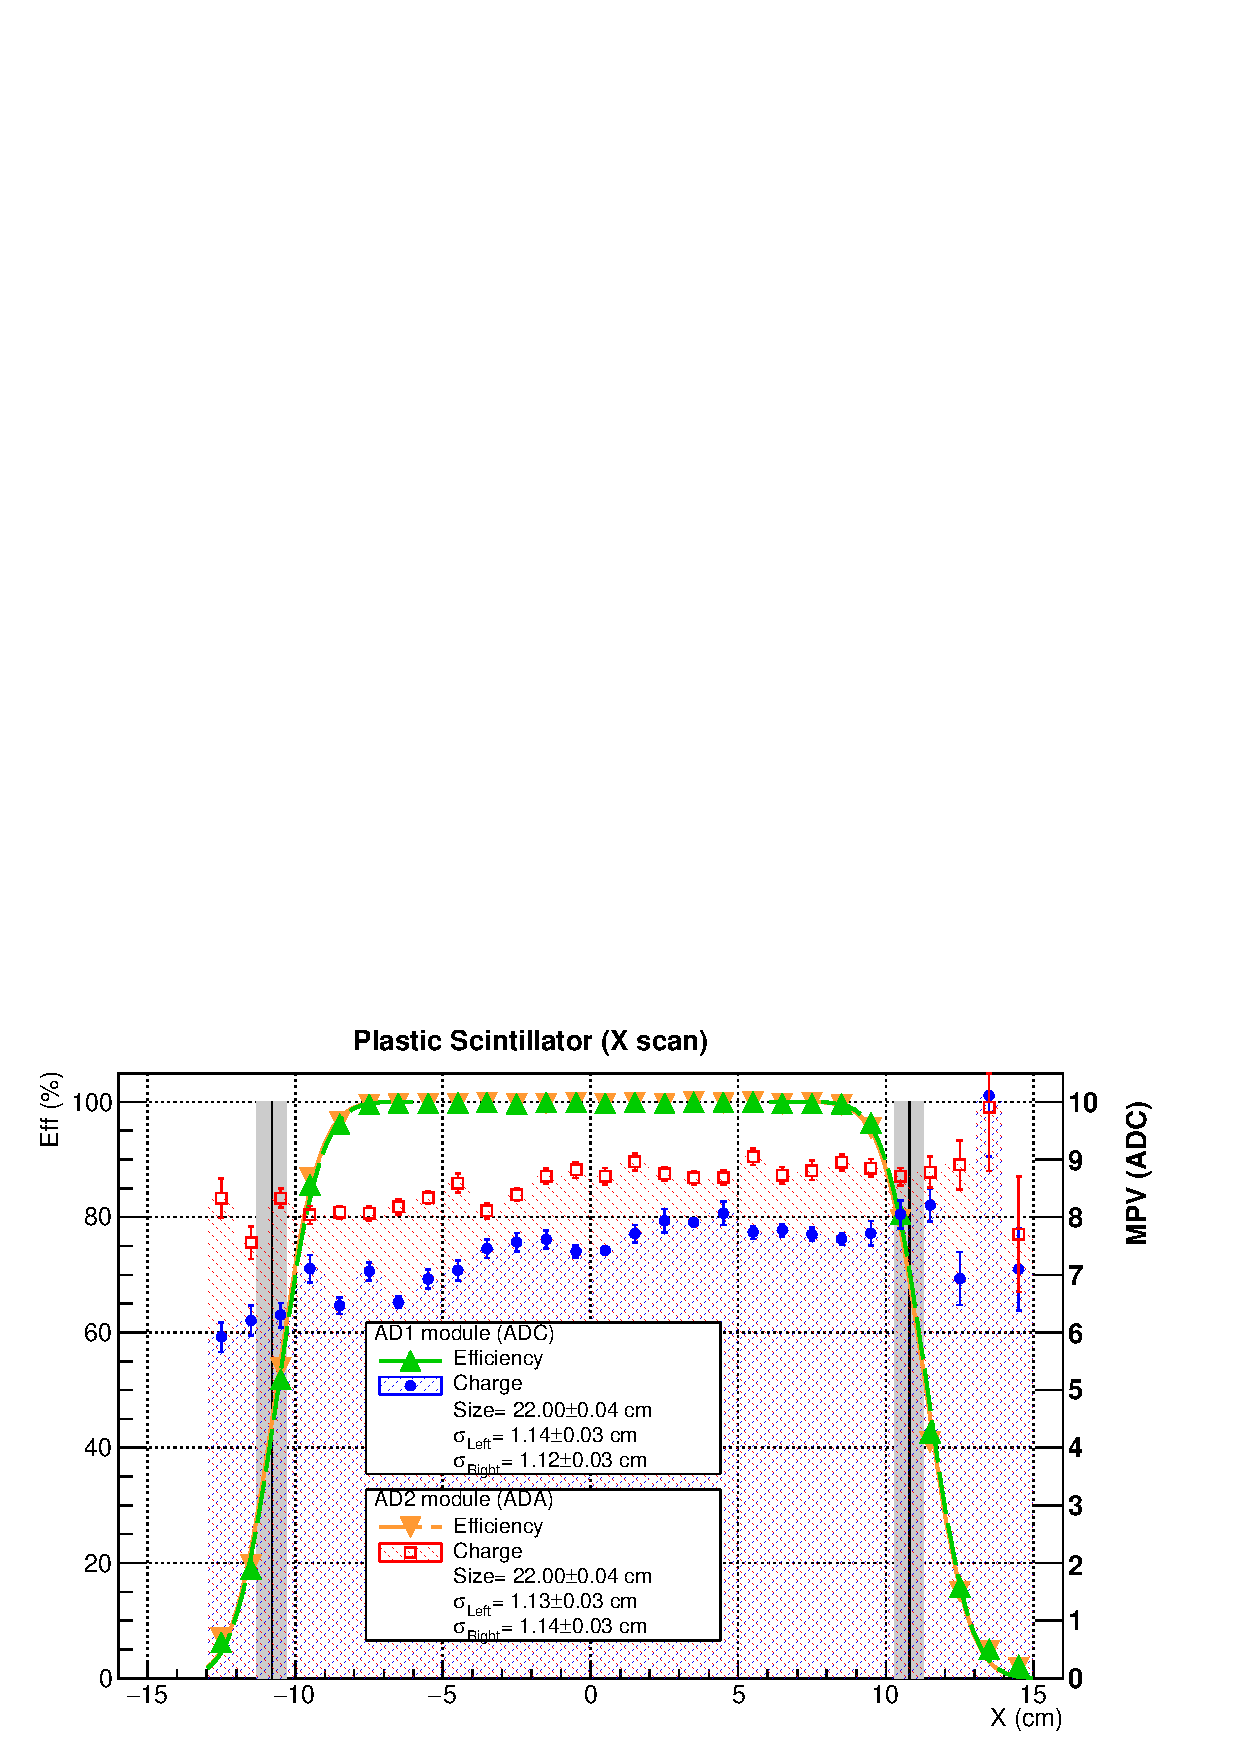
\includegraphics[scale=0.5]{./images/scan/Xaxis_scan.pdf}
			\caption{
				Charge and efficiency obtained in the X-axis scan along the center of the ADs modules.
				%Scan of AD module from the plastic scintillator center along the $X$-axis (horizontal).
			}
			\label{figure:ScanX-ADcenter}
		\end{center}
	\end{figure}
	
	\begin{figure}[h!]
		\begin{center}
			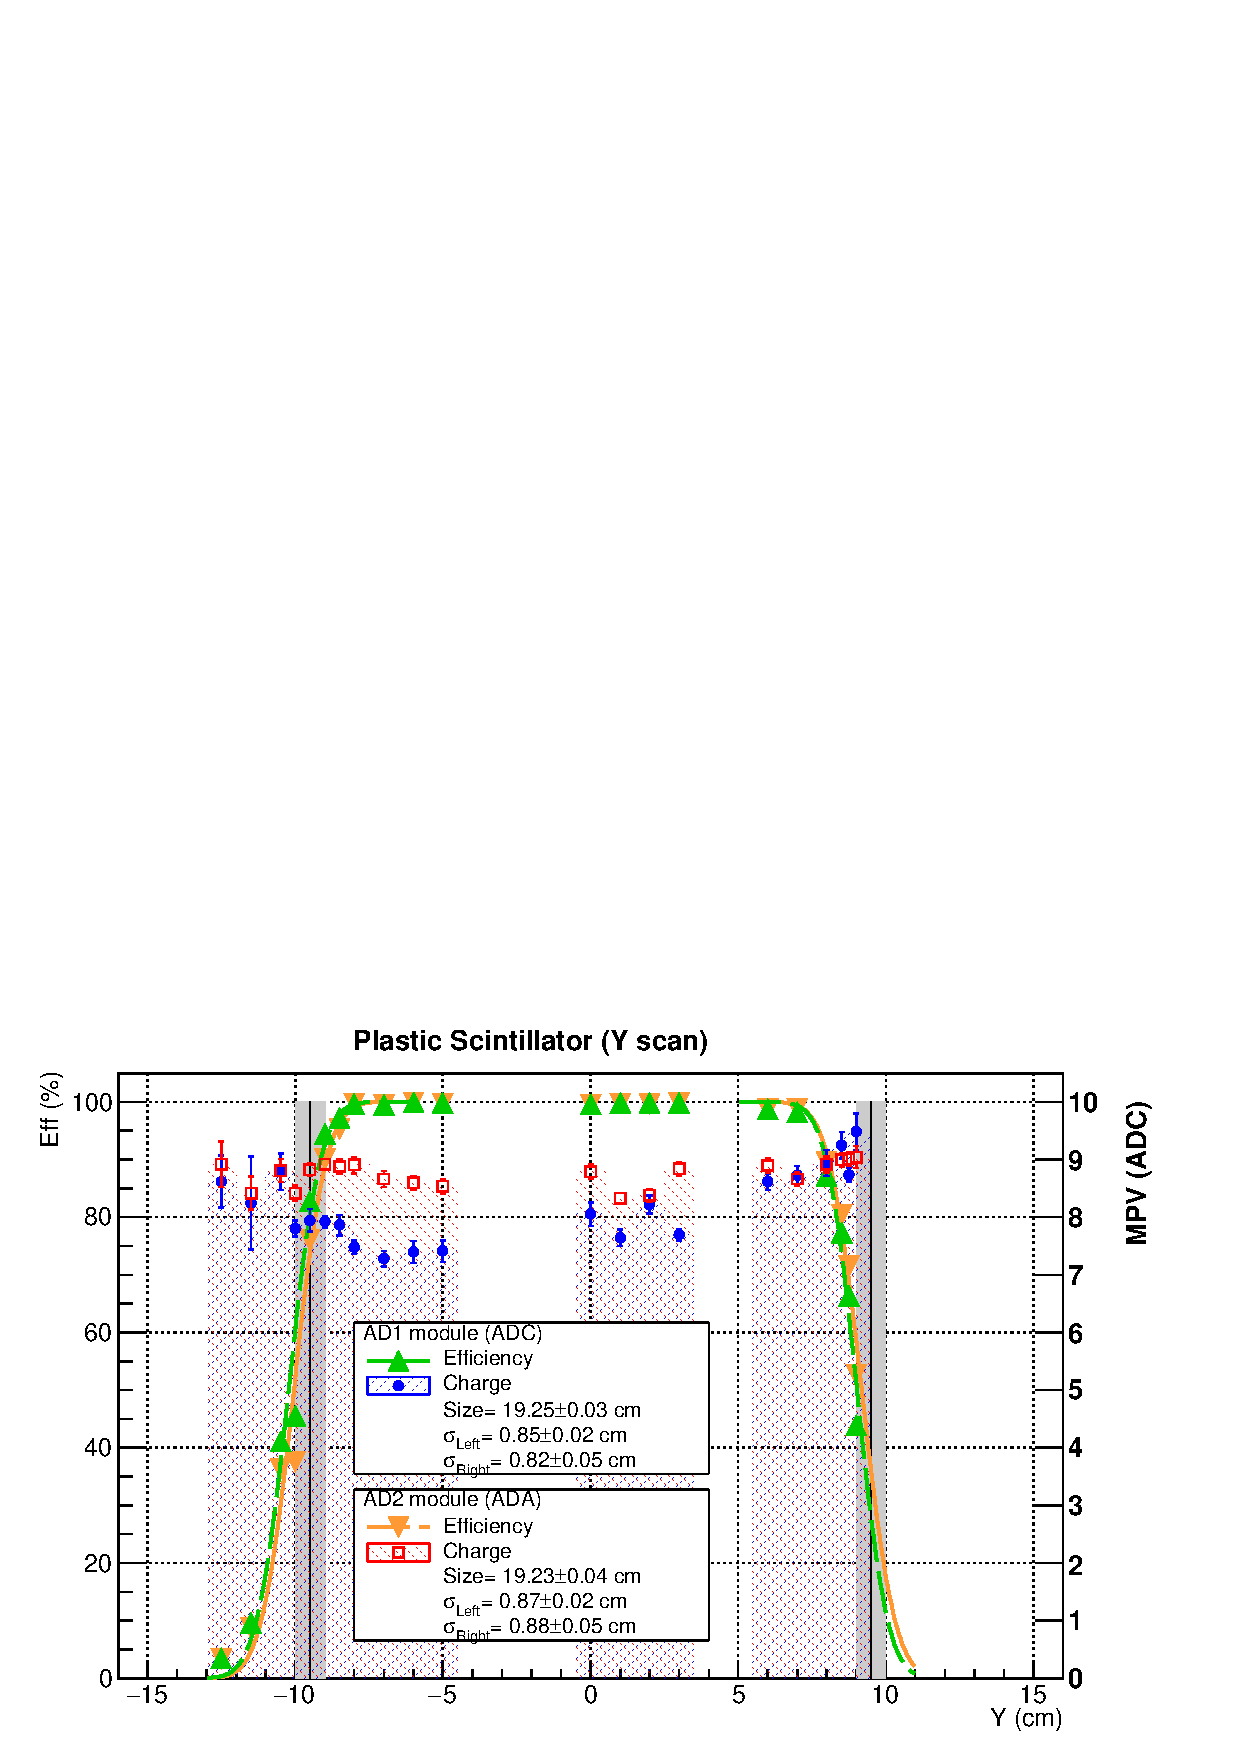
\includegraphics[scale=0.5]{./images/scan/Yaxis_scan.pdf}
			\caption{Scan of AD module from the plastic scintillator center along the $Y$-axis (horizontal). 
				%The empty spaces are due we  the measurements in those places.
				The empty spaces in the plots are skipped measurements.
				}
			\label{figure:ScanY-ADcenter}
		\end{center}
	\end{figure}
	%
	To estimate the position of the borders and the size of the  beam a \textit{Gaussian Cumulative Function distribution} (CDF), shown in the 
	equation \ref{eq:cdf}, was adjusted to the edges of the efficiency plots.
	
	\begin{equation} \label{eq:cdf}
	F(X|\mu,\sigma)=\frac{1}{\sigma\sqrt{2\pi}} \displaystyle \int_{-\infty}^{X}
	e^{\frac{-(t-\mu)^{2}}{2\sigma^{2}}} \, dt
	\end{equation}
	%
	The physical lengths in the vertical and horizontal axes of both modules were calculated using the differences between the distances of the mean values of CDF for each case, obtaining a length of $X$=22 and $Y$=19 cm for each axis, that are consistent with the physical length.
	The size of the beam calculated using the sigmas of the CDF are $\sigma_{Y}=1.13\pm 0.06$ cm and $\sigma_{X}=0.86\pm0.08$ cm. %
	The scan in the optical connectors demonstrates that the detection probability is very low, the light here is mainly produced by cherenkov effect, that is rapidly absorbed by the optical fibre. %
	The results of the performance of this section can be seen in Figure \ref{figure:ScanConn}.
	
	\begin{figure}[h!]
		\begin{center}
			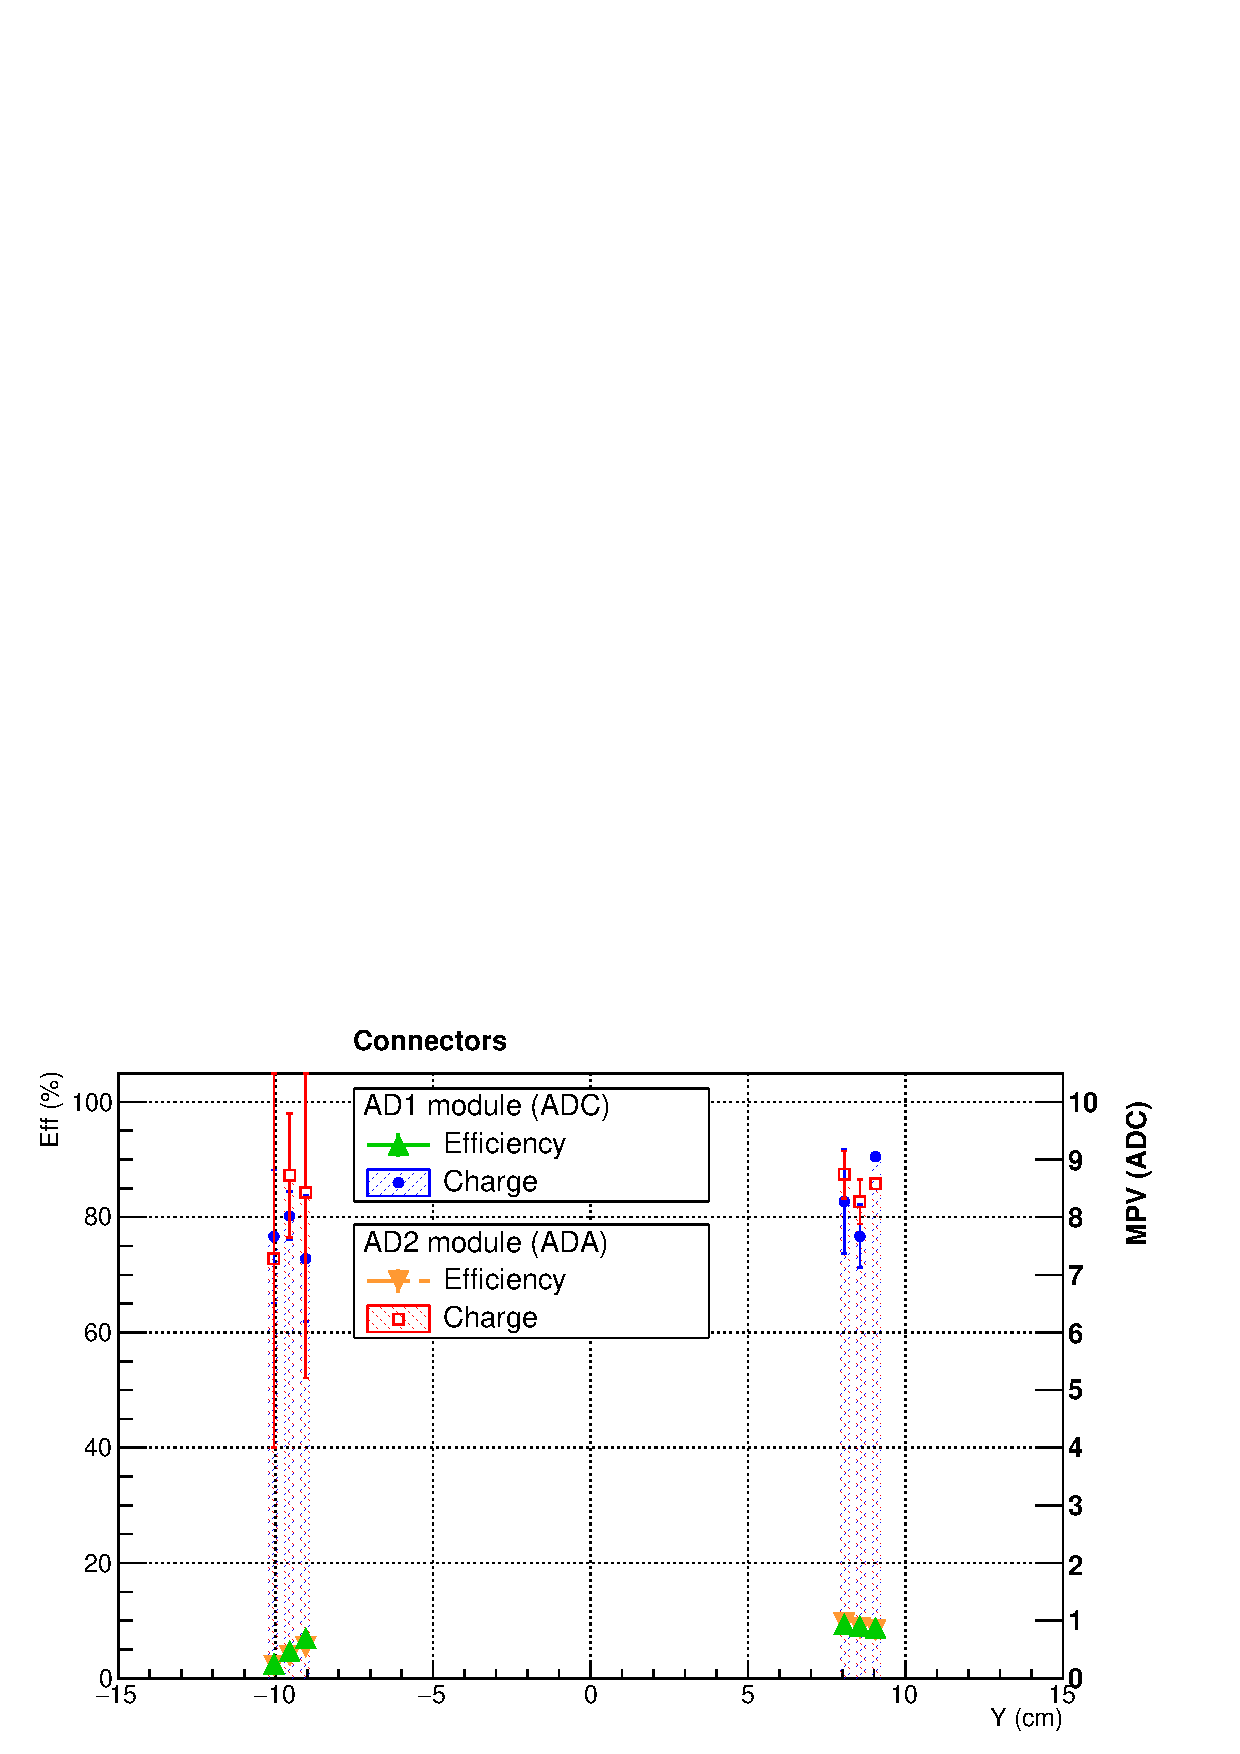
\includegraphics[scale=0.5]{./images/scan/Connectors_scan.pdf}
			\caption{Scan of two optical connectors of the ADA and ADC modules ($y$-axis scan)}
			\label{figure:ScanConn}
		\end{center}
	\end{figure}
	%
	The efficiency when the beam hits in the bunch of fibres (see Figure \ref{figure:ScanFib}) shows that the detection efficiency is low and a few events are detected. The bunch of fibres is glued in a cylindrical and transparent connector made of acrylic and coupled to the PMT photochathode. Therefore, when a particle hits the connector ($\sim$2.5 cm away from the PMT photochathode) cherenkov light is produced and reach the photocathode of the PMT; if we move the beam in the vertical axis we expect a reduction in the efficiency because there is less material. The charge measured in this section is only due the cherenkov light that reach the photocathode \cite{ClearFib-performace}.
	%
	The efficiency along the PMT is reduced when a particle hits far from the photocathode and should produce a 
	signal when impact in the photocathode or the dynodes. This can be seen in Figure \ref{figure:scanPMT}. %
	The photocathode is placed in the most left side of the plot. As is expected a significant efficiency of 40\% 
	is observed when particles hits the PMT photochathode.
	
	\begin{figure}[h!]
		\begin{center}
			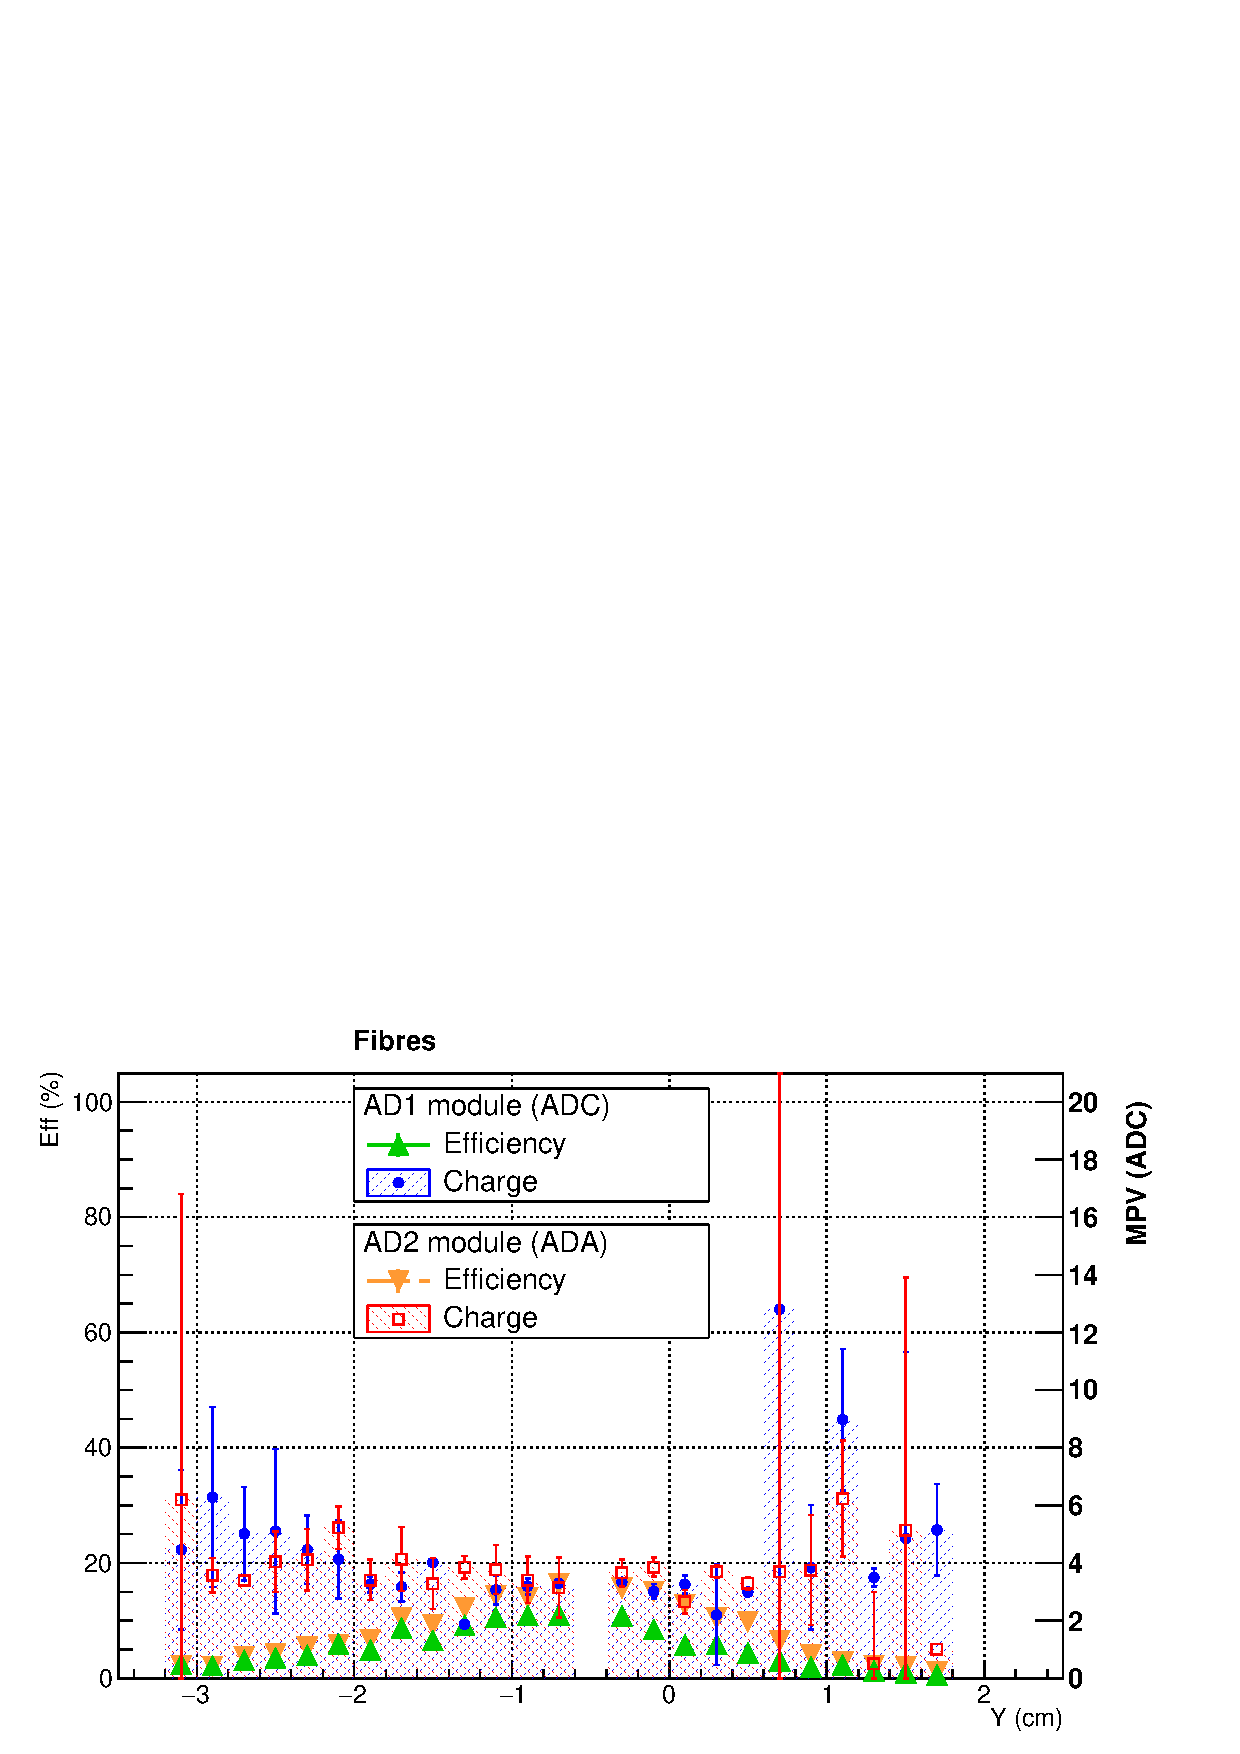
\includegraphics[scale=0.5]{./images/scan/Fiber_scan.pdf}
			\caption{Scan of bunch of fibres for ADA and ADC modules ($y$-axis scan).}
			\label{figure:ScanFib}
		\end{center}
	\end{figure}
	
	\begin{figure}[h!]
	\begin{center}
	  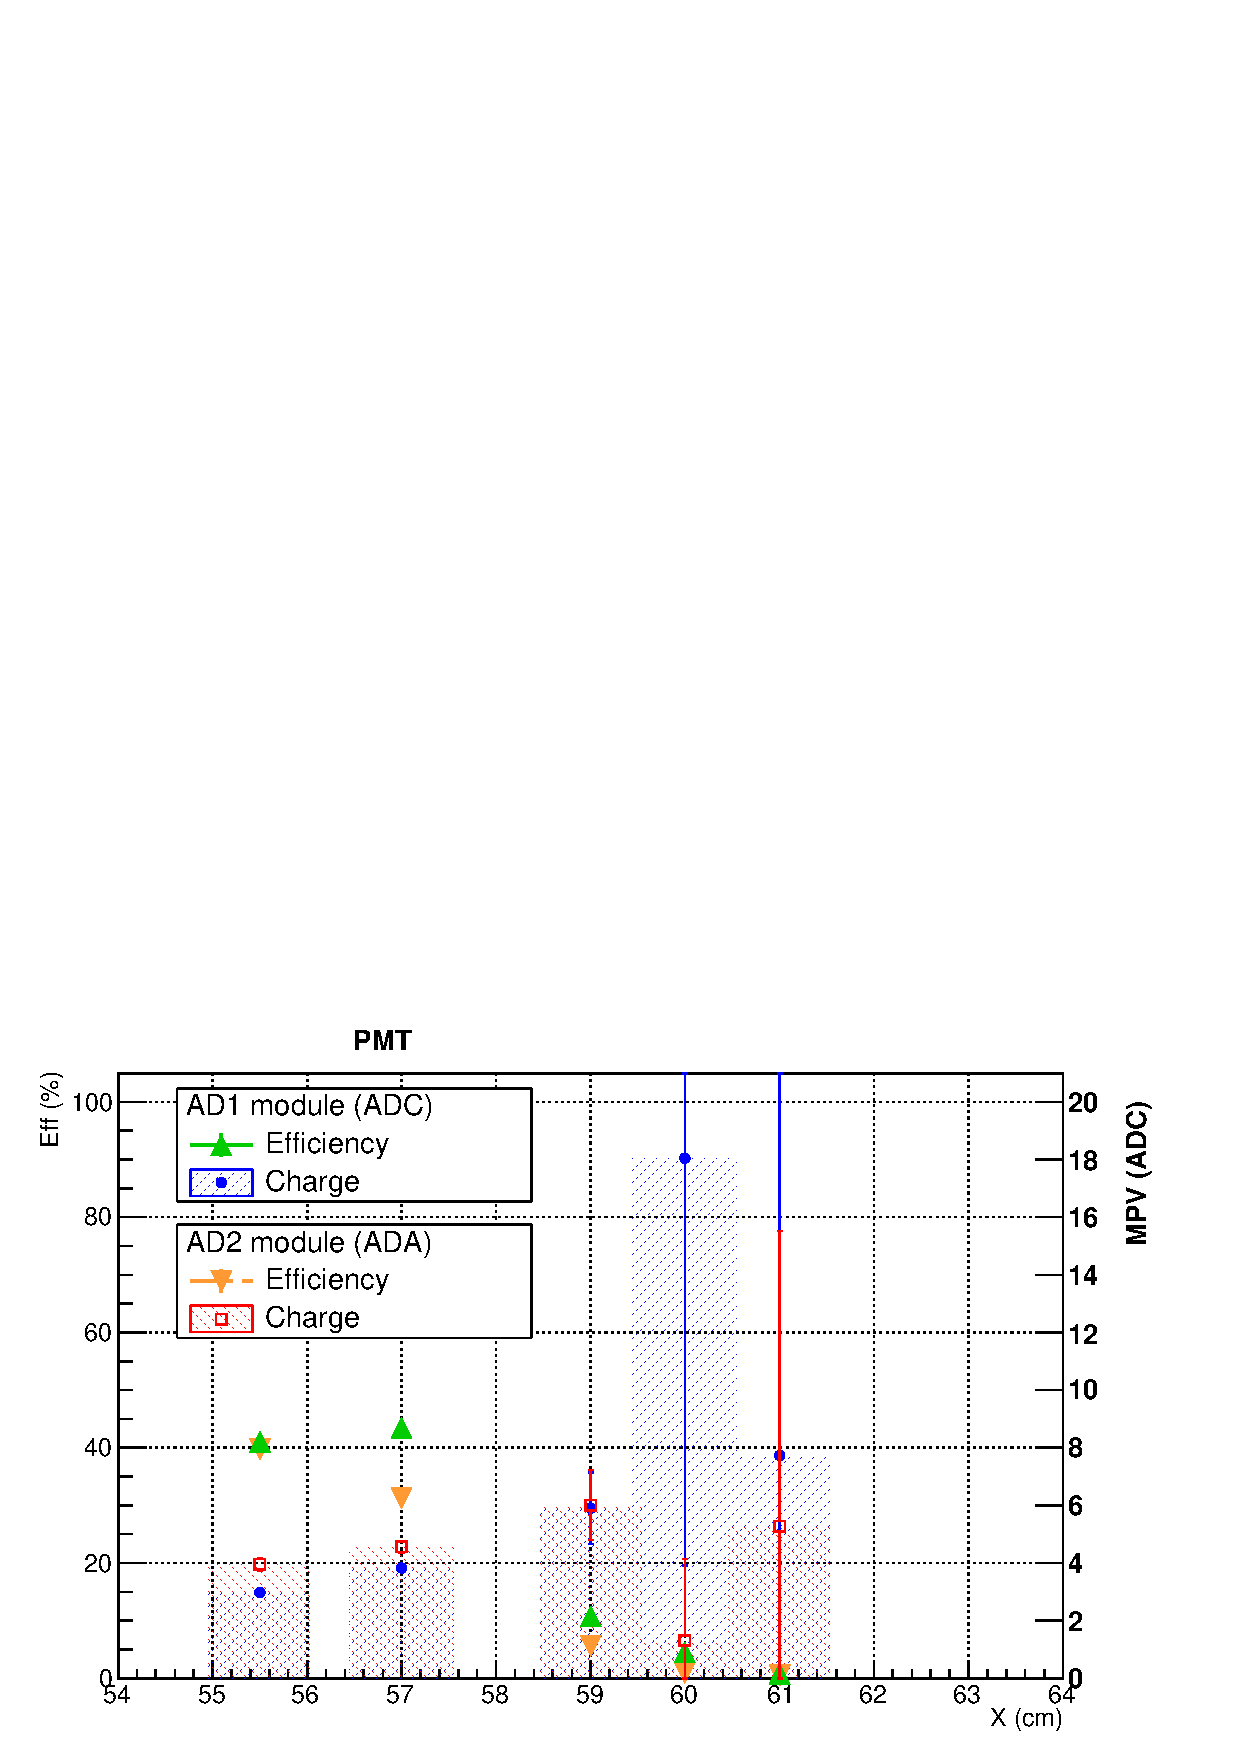
\includegraphics[scale=0.5]{./images/scan/PMT_scan.pdf}
	  \caption{PMT scan for ADA and ADC modules ($x$-axis scan).}
	  \label{figure:scanPMT}
	\end{center}
	\end{figure}

	\subsection{Time analysis.}\label{section:TimeMeasurement}
	
	To analyze the time response of the detectors, we use all the detectors placed in the setup and 
	define a time reference, given that the particles coming from the PS arrives randomly. %
	The T0-end detector was chosen because of its good time resolution ($\sim$50 ps)\cite{T0detector} and the 
	distances respect to other detectors is suitable to distinguish pions and protons using the \textit{Time Of 
	Flight} technique.
	%
	For analyze and select particles we used the time differences between the Black-start and T0-end detectors.
	Two time windows were defined, one to select pions and another for protons. %
	This is shown in Figure \ref{figure:ParSel_1GeV}, pions were selected from 62.0 to 71.5 ns (gray
	histogram) and protons from 71.5 to 76.0 ns (yellow histogram). 
	This strategy will allow us to identify the particles in other detectors even if the particles are overlapped.
	
	\begin{figure}[h!]
	  \begin{center}
		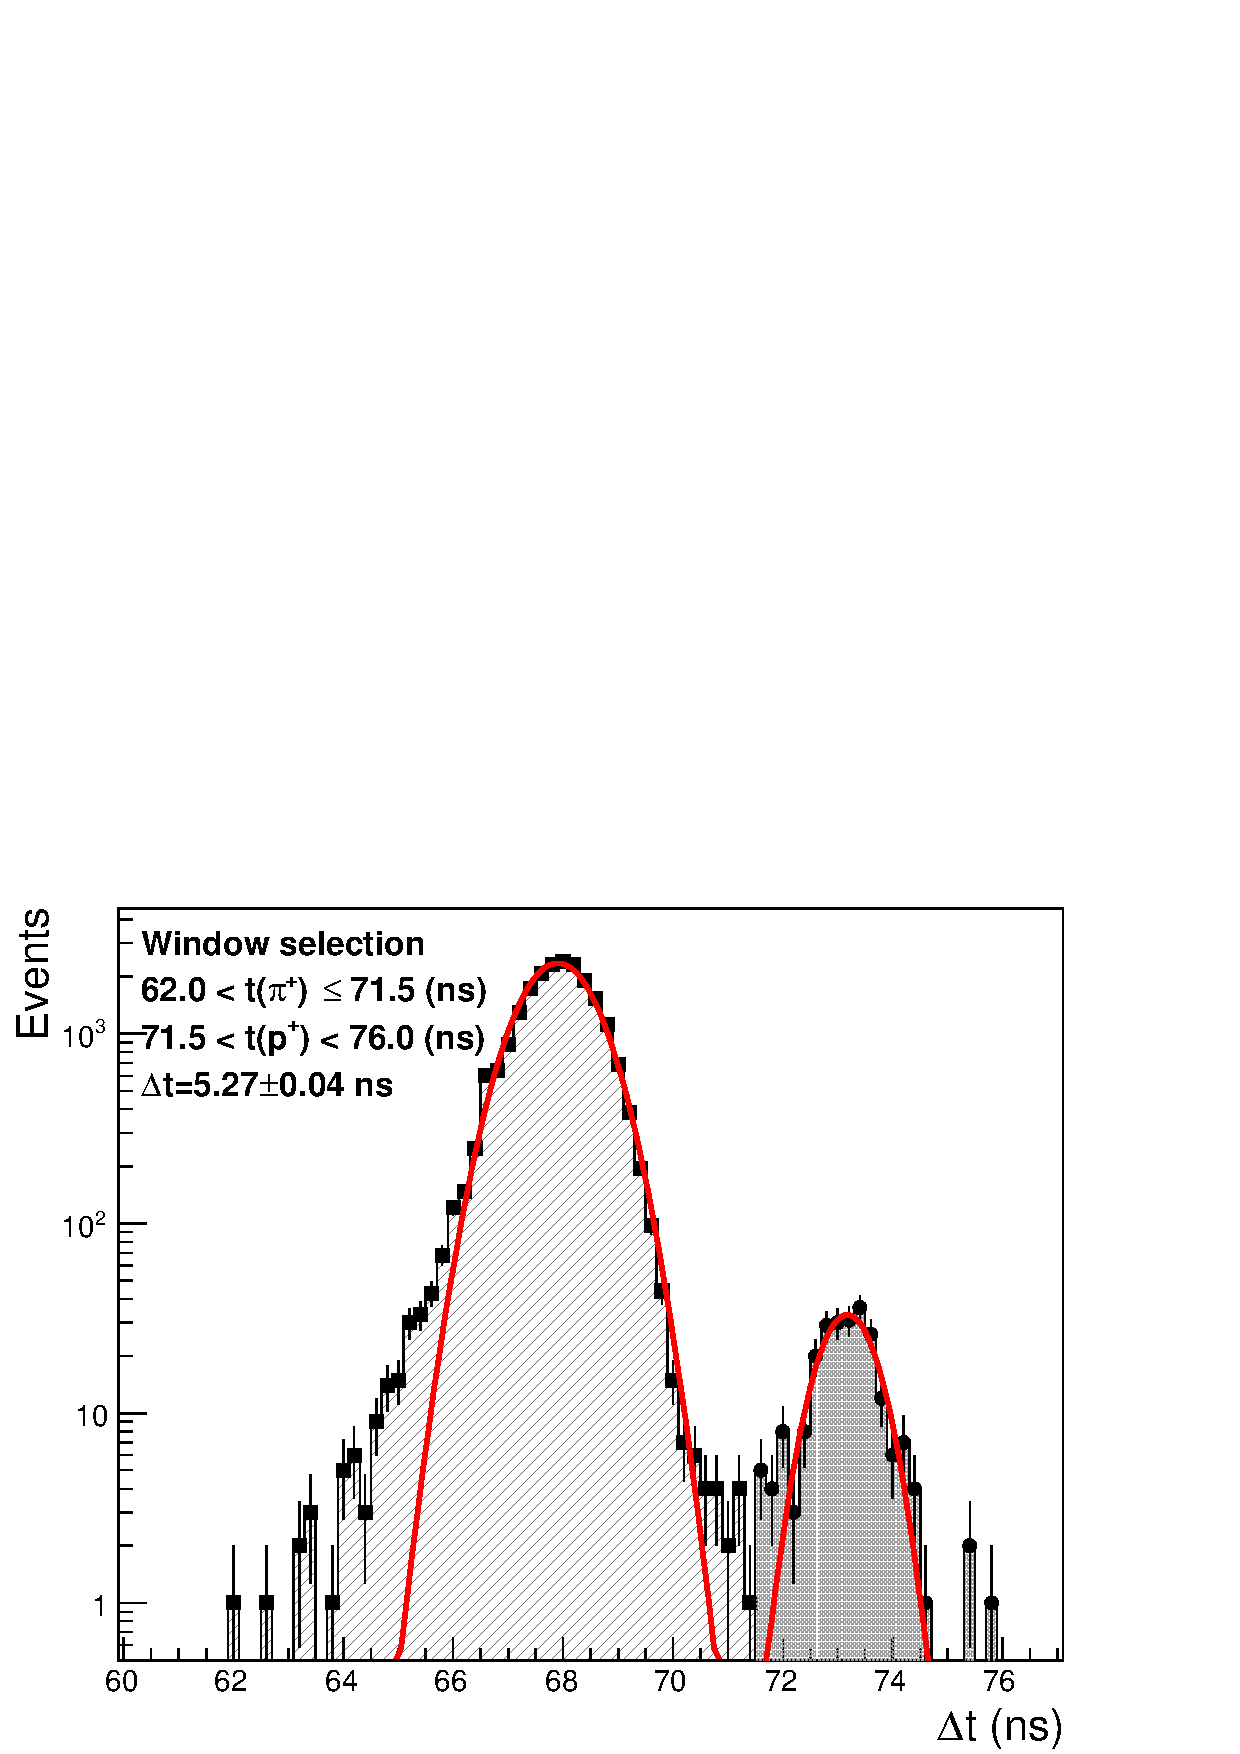
\includegraphics[scale=0.50]{./images/time/1GeV/NotepPiSelH1.pdf}%NotepPiSelH1_1GeV.pdf}
		\caption{Time window to select pions(gray) and protons(yellow). The time difference between Black-start and T0-end detectors
		was used, due the good separation and statistic provided by this configuration.}
		\label{figure:ParSel_1GeV}
	  \end{center}
	\end{figure}
	
	\begin{figure}[h!]
	  \begin{center}
	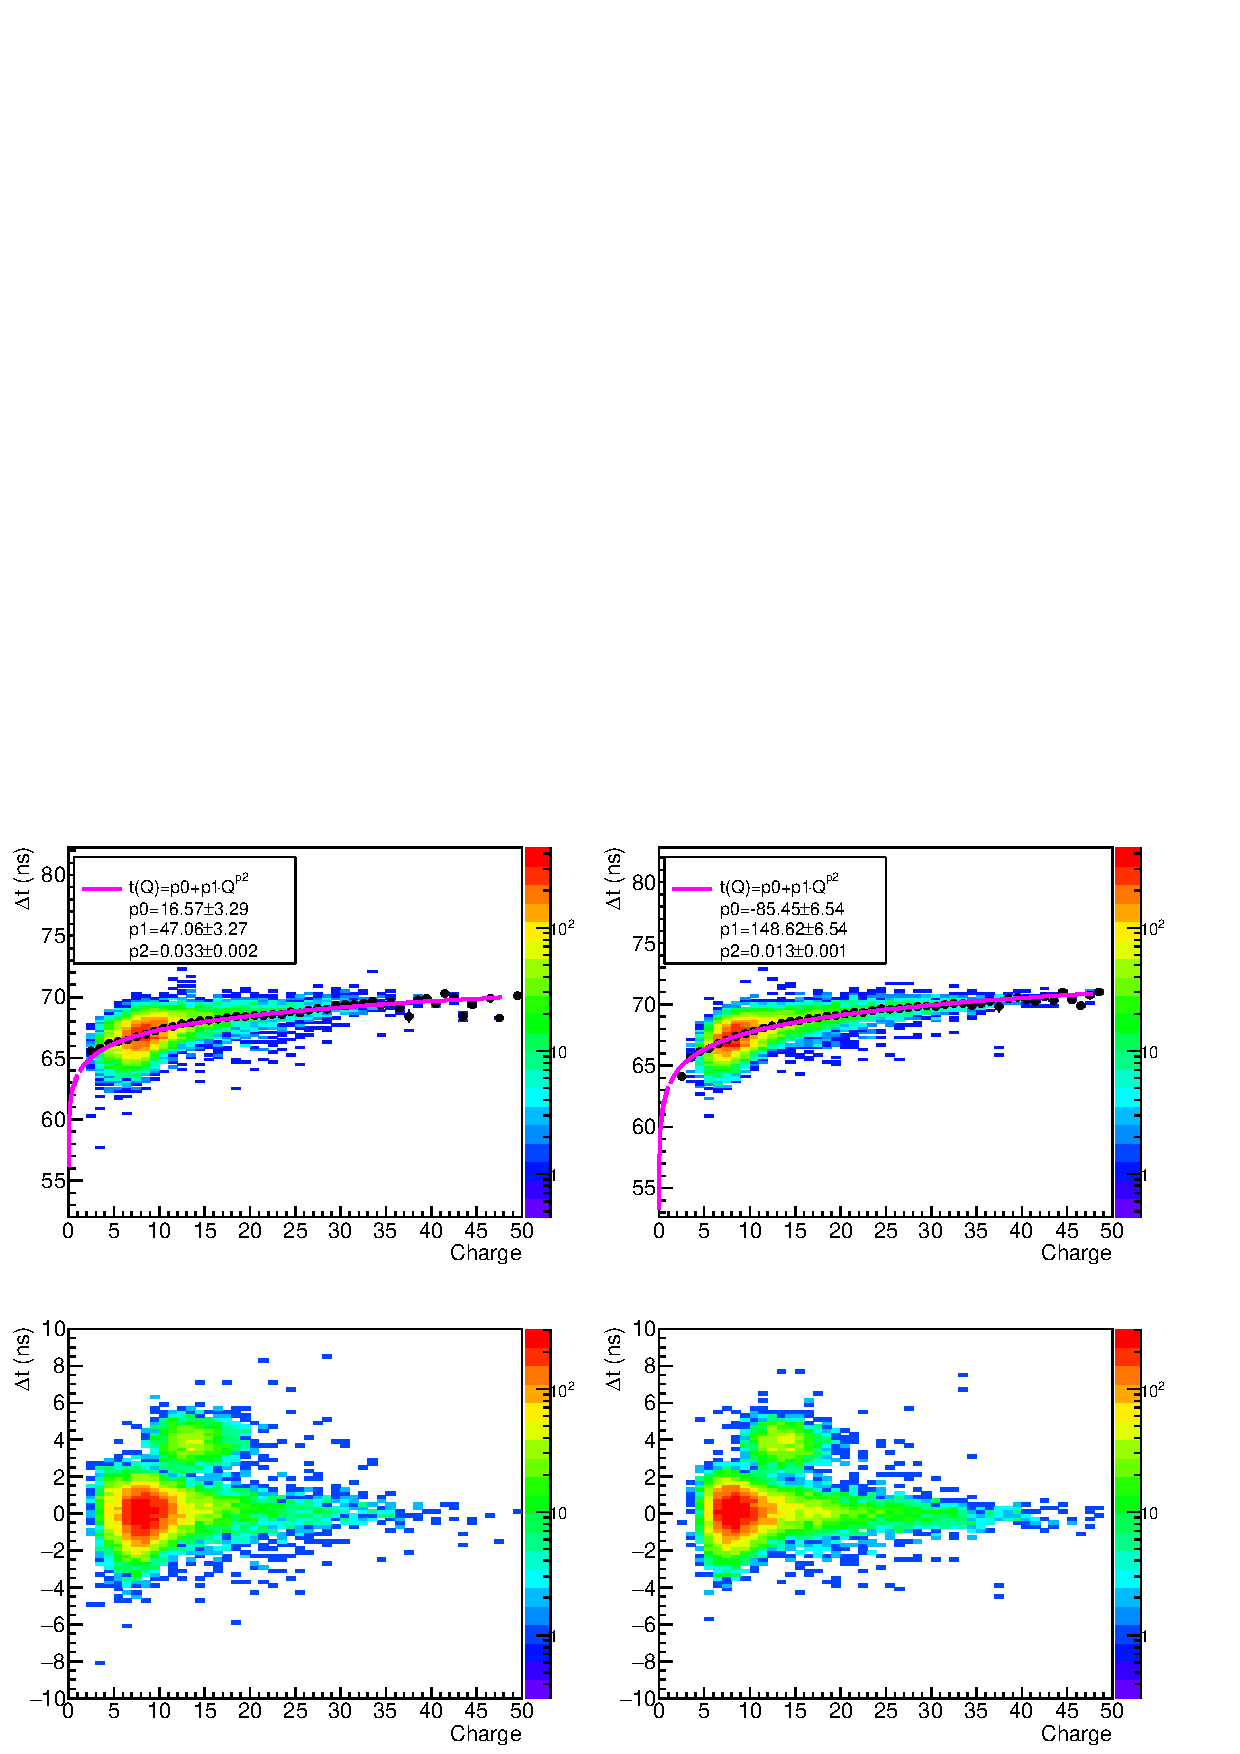
\includegraphics[scale=0.60]{./images/time/1GeV/NoteSlewH2.pdf}%NoteSlewH2_1GeV.pdf}
	\caption{Time slewing correction calculated using the pions distributions of AD1 and AD2 (top row).The corrected distribution
	was obtained as can be seen in the bottom row.}
	\label{figure:TimeQSlew_1GeV}
	  \end{center}
	\end{figure}
	
	%\subsubsection{Time slewing correction.}
	%
	The time measurement are affected by
	an slewing effect and can be corrected applying the time slewing correction technique to improve the measurement \cite{V0Performance}. The distribution for pions was selected to make the correction because the
	effect is clearest. In the Figure \ref{figure:TimeQSlew_1GeV} can be seen the profile of the time with respect
	to the charge, represented by the black dots; the behavior can be parametrized according to 
	$t(Q)=p0+p1\cdot Q^{p2}$ where $p0$, $p1$, and $p2$ are constants parameters. Once we have obtained the parameters
	from the fit, the time corrected is calculated subtracting the time $t(Q)$ to the measured time 
	$ t(\textrm{corr.})=t(\textrm{measured})-t(Q)$, where $t(\textrm{corr.})$ is the time corrected and
	$t(\textrm{measured})$ is the time measured of each individual event. The corrected distributions are shown in Figure \ref{figure:Time_1GeV} (bottom histograms),  and show how the slewing effect has disappeared. In Figure
	\ref{figure:Time_1GeV} can be compared the time response of the modules before (top row) and after (bottom
	row) the slewing correction.% 
	
		%%----------------------------------------------------------------------------
		\begin{figure}[h!]
			\begin{center}
				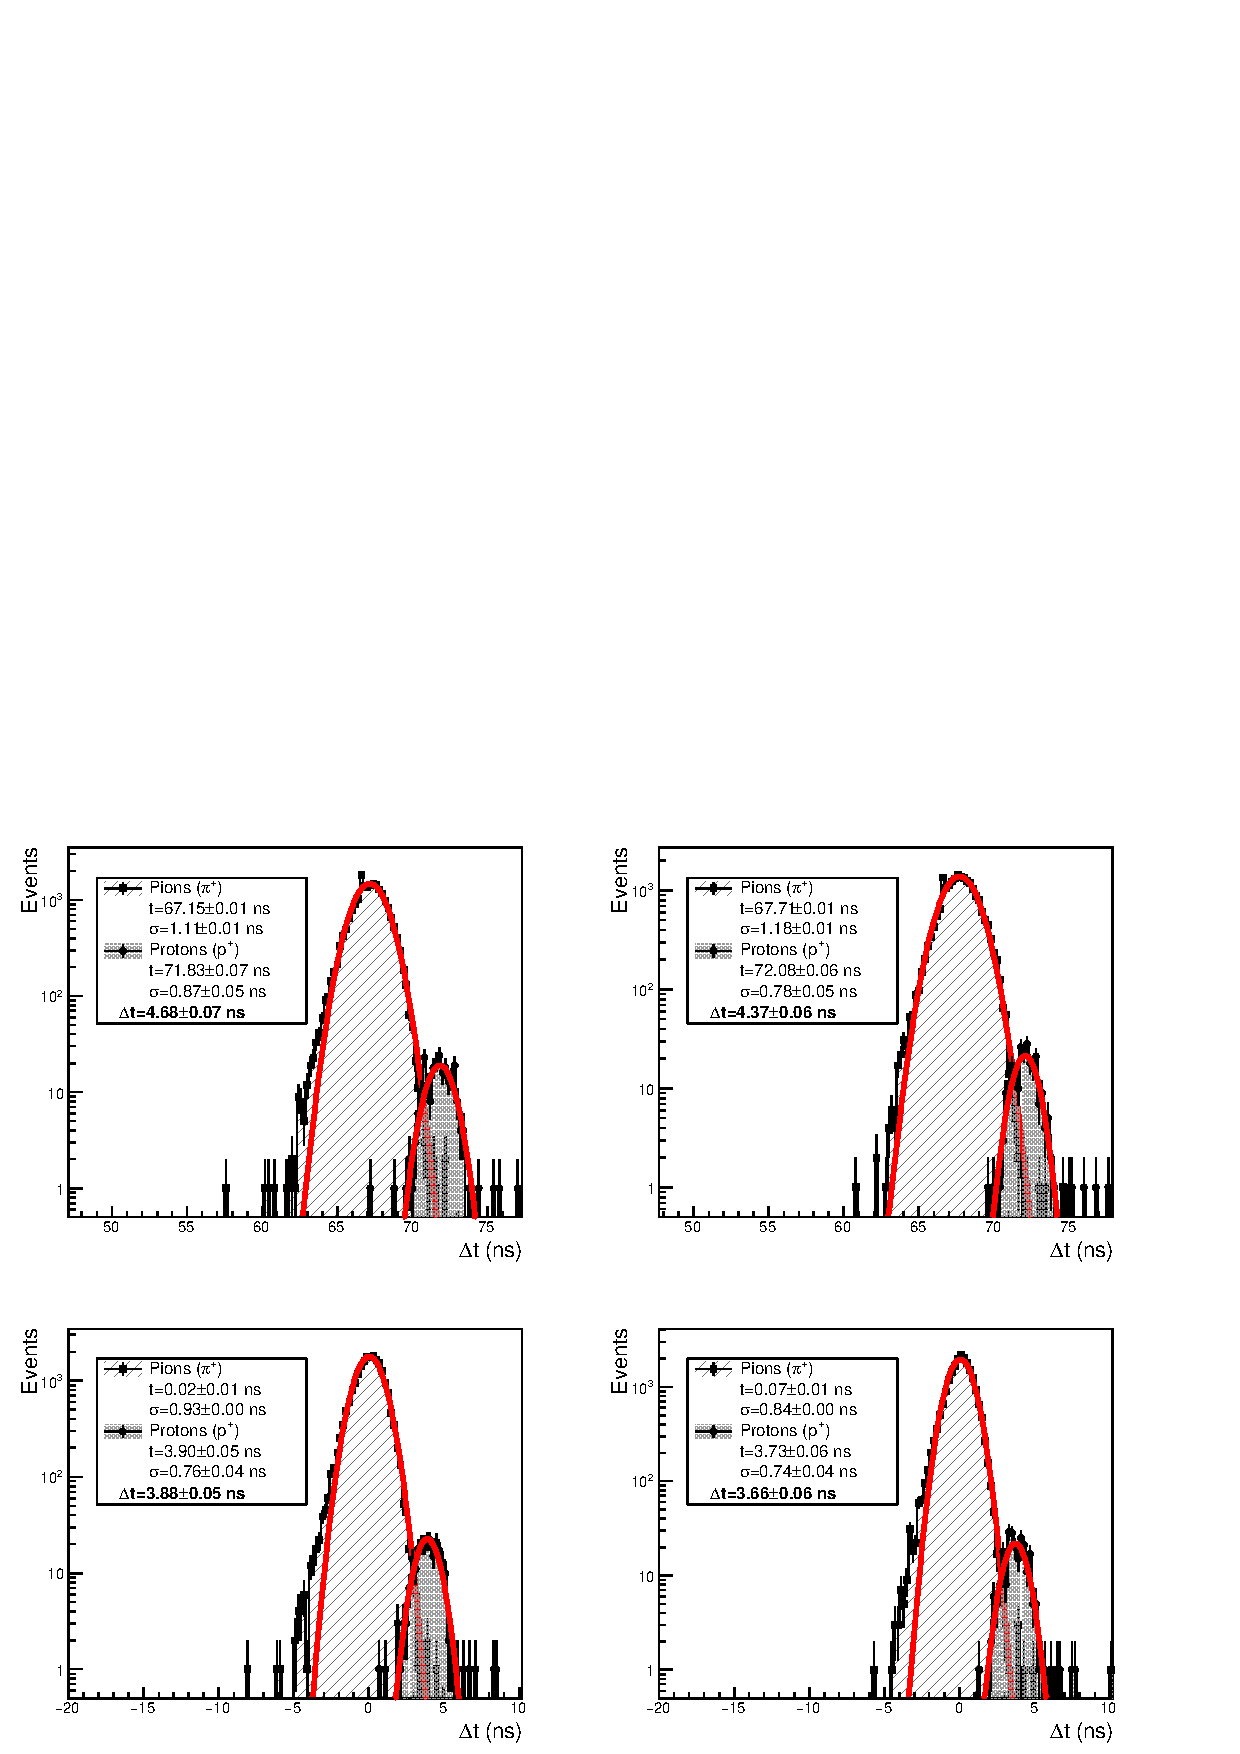
\includegraphics[scale=0.70]{./images/time/1GeV/NoteSlewH1.pdf}%NoteSlewH1_1GeV.pdf}
				\caption{Time distributions of pions (gray) and protons (yellow) at 1 GeV/c beam momentum of ADs detectors before (top row) and
					after (bottom row) the time slewing correction and the time of flight difference	 measurements.}
				\label{figure:Time_1GeV}
			\end{center}
		\end{figure}
	
	%\subsubsection{Time of flight.}
	The materials placed along the experimental setup plays an important role in the analysis for particle 
	identification, i.e. to analyze the time and charge properties. AD detector is composed mainly by a piece of
	\textit{Bicron 404} \cite{BC404_Manual} plastic scintillator of 2.5 cm of thickness; the same kind of material
	is assumed for the Black hodoscopes but with a thickness of 4 cm. The T0 Cherenkov radiators have a more
	complex composition, and is formed by a 2 cm of thickness quartz radiator \cite{T0detector}, for the PMT glass
	of the vacuum tube and the aluminum cover we will consider 1 mm in the front and 1 mm more in the back, and
	finally the 16 dynodes are made of 0.1 mm thick iron (Fe).
	
	%\subsection{Deposition of energy calculation.}
	The energy deposited by the particles in the detector is translated to an amount of charge measured, using
	this we obtained a calibration of the energy deposition in the material. %
	For detectors of moderate thickness $x$, e.g. scintillators or LAr cells, the energy loss probability 
	distribution is adequately described by the highly-skewed Landau (or Landau-Vavilov) distribution 
	\cite{ReviewPDG, Grupen} where the most probable energy loss is:
	
	\begin{equation}\label{eq:landauMPE}
	\Delta_p=\xi\left( \ln \frac{2mc^2 \beta^2 \gamma^2}{I}
	+ \ln\frac{\xi}{I}+j+\beta^2-\Delta(\beta\gamma) \right)\,\,\,\, \text{and} \,\,\,\, \xi=\frac{K}{2} \frac{Z}{A}z^2(x/\beta^2)
	\end{equation}
	
	The new energy and momentum of the particle was recalculated on each stage using the material budget and
	$E^2=p^2c^2+M^2c^4$. %
	For practical reasons we have defined five stages in the beam setup, which are listed in the Table
	\ref{table:stages}. 

	\begin{table*}[!h]
		\centering
		\scalebox{0.87}{
			\begin{tabular}{|c||c|c|}
				\hline
				Stage &  Placement & Distance (cm) \\ \hline
				s0 & Before Black-start& - \\
				s1 & Black-start to AD1& 65.5 \\
				s2 & AD1 to AD2& 3.0\\
				s3 & AD2 to T0-start& 240.5 \\
				s4 & T0-start to T0-end& 62.0 \\
				s5 & T0 end to Black-end& 854.0 \\
				\hline
			\end{tabular}
		}
		\caption{Stages: labels, placement and distances traveled by the particles along them. The distances where taken from the middle of each scintillator and the middle of the crystal of the T0s.}
		\label{table:stages}
	\end{table*}
	%
	The energy loss has been calculated for pions and protons taking into account the material budget
	of each detector to obtain the new momentum of the particle in each stage.  This loss leads to
	an increase on the time of flight difference between pions and protons which have been calculated 
	for each stage using:
	
	\begin{equation}
	t_j=\frac{L}{\beta c}=\frac{L}{p_j c}\sqrt{p_j^2+m_j^2c^2}
	\end{equation}
	%
	where $j$ indicate the particle (pion or proton for example) and $L$ the distance traveled. The time of 
	flight difference $\Delta t$ is calculated subtracting the time of flight of two different particles
	traveling the same distance.
	
	\begin{equation}\label{eq:tof}
	\Delta t= t_1-t_2= \frac{L}{c}\left[\left(1+\frac{m_1^2c^2}{p^2_1}\right)^{1/2}- \left({1+\frac{m_2^2c^2}{p^2_2}}\right)^{1/2} \right]
	\end{equation}
	
	The results are summarized in the Tables\ref{table:1GeVtimes}, \ref{table:1p5GeVtimes}
	and \ref{table:2GeVtimes} for a momentum of 1, 1.5 and 2 GeV/c respectively. The measurements have a good
	agreement with respect to the theoretical calculations; and the time slewing correction is improved in
	comparison with the not corrected data.
	
	%% Table for 1 GeV/c time of flight
	\begin{table}[h!]
		\centering
		\begin{tabular}{ | c|| c || c c c| } \hline
			\textbf{Detector} & Distance (cm) &Theoretical $\Delta t$ (ns) &$\Delta t$ (ns) &Slewing corr. $\Delta t$ (ns) \\ \hline\hline
			
			AD1	    &305.5	&4.067	&4.68$\pm$0.07	&3.9$\pm$0.05	\\
			AD2	    &302.5	&4.030	&4.37$\pm$0.06	&3.66$\pm$0.06	\\
			T0.start      &62.0	&0.907	&1.18$\pm$0.04	&-		\\
			Black.start   &371.0	&4.882	&5.27$\pm$0.04	&4.66$\pm$0.03	\\
			Black.end     &845.0	&13.438	&14.29$\pm$0.09	&14.5$\pm$0.07\\ \hline
			%4.067	4.030	0.907	4.882	13.438
			\hline
		\end{tabular}
		\caption{Distances, theoretical and measured time of flight differences between pions and protons respect
			to T0-end detector for 1 GeV/c beam momentum. The measured time of flight before and
			after apply the time slewing correction are in the fourth and fifth columns respectively.
			}
		\label{table:1GeVtimes}
	\end{table}

	%% Table for 1.5 GeV/c time of flight
	\begin{table}[h!]
	\centering
	\begin{tabular}{ | c||c c c| } \hline
		\textbf{Detector} &Theoretical $\Delta t$ (ns) &$\Delta t$ (ns) &Slewing corr. $\Delta t$ (ns) \\ \hline\hline
		
		AD1	    &1.809	&2.03$\pm$0.08	&1.83$\pm$0.09	\\
		AD2	    &1.791	&1.2$\pm$0.1	&1.68$\pm$0.08	\\
		T0-start      &0.394	&0.14$\pm$0.01	&-		\\
		Black-start   &2.200	&2.1$\pm$0.03	&2.11$\pm$0.02	\\
		Black-end     &5.824	&6.12$\pm$0.04	&6.29$\pm$0.03 	\\ \hline
		%1.809	1.791	0.394	2.200	5.824
		\hline
	\end{tabular}
	\caption{Theoretical and measured time of flight differences of pions and protons respect
		to the T0-end detector at 1.5 GeV/c beam momentum. %
		The measured time of flight before and
		after apply the time slewing correction are in the third and fourth columns respectively.}
	\label{table:1p5GeVtimes}
	\end{table}

	%% Table for 2 GeV/c time of flight
	\begin{table}[h!]
	\centering
	\begin{tabular}{|c||c c c|} \hline
		\textbf{Detector} &Theoretical $\Delta t$ (ns) &$\Delta t$ (ns) &Slewing corr. $\Delta t$ (ns) \\ \hline\hline
		
		AD1	    &1.010	&0.72$\pm$0.04	&0.66$\pm$0.04	\\
		AD2	    &1.000	&0.14$\pm$0.5	&0.54$\pm$0.04	\\
		T0-start      &0.218	&1.0$\pm$0.01	&-		\\
		Black-start   &1.233	&1.19$\pm$0.02	&1.09$\pm$0.02	\\
		Black-end     &3.288	&3.21$\pm$0.09	&3.77$\pm$0.01\\ \hline
		\hline
	\end{tabular}
	\caption{2 GeV/c beam momentum theoretical and measured time of flight differences between pions and protons respect
		to the T0-end detector. The measured time of flight before and
		after apply the time slewing correction are in the third  and fourth columns respectively.}
	\label{table:2GeVtimes}
	\end{table}
	
	\begin{figure}[h!]
	  \begin{center}
	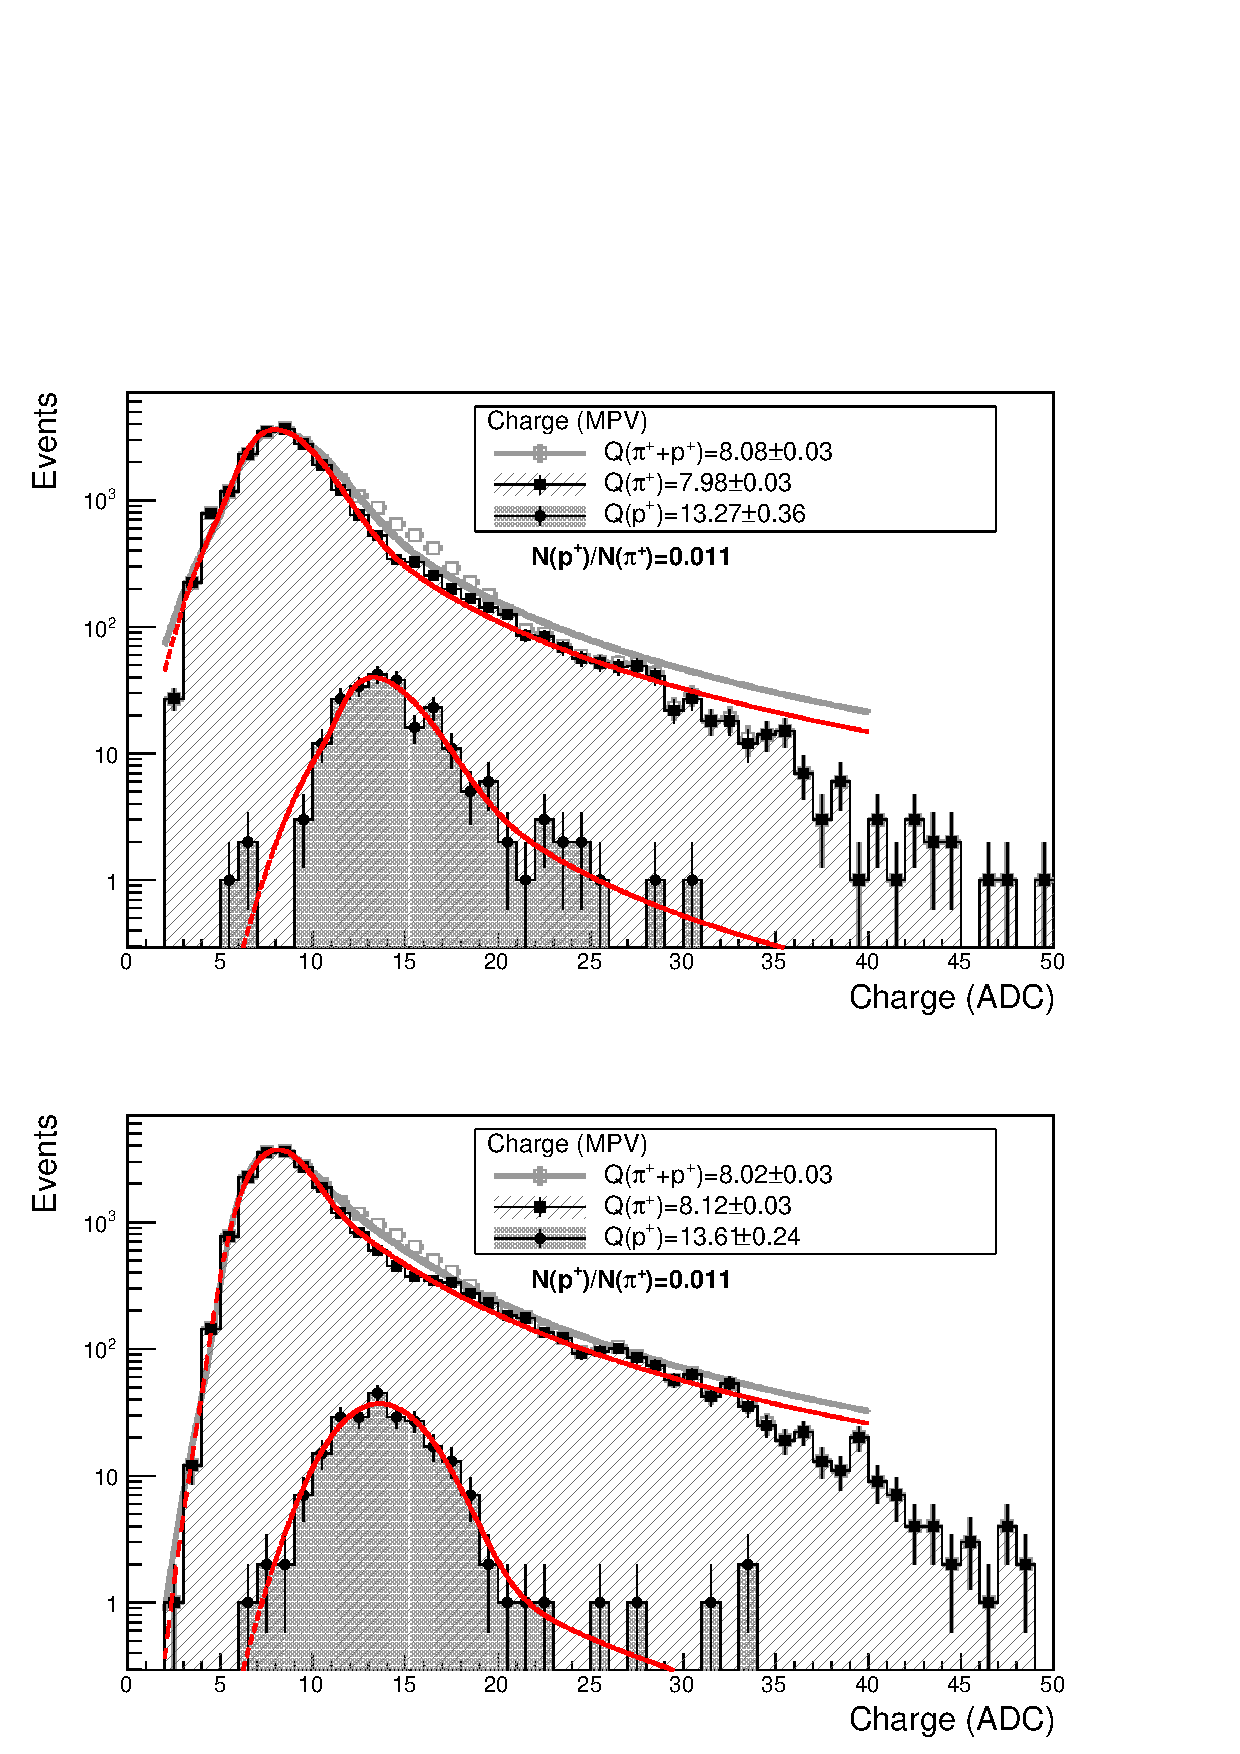
\includegraphics[scale=0.70]{./images/time/1GeV/NoteQ.pdf}%NoteQ_1GeV.pdf}
	\caption{Charges distributions for 1 GeV/c beam momentum for all particles and pions and protons separated.}
	\label{figure:Q_1GeV}
	  \end{center}
	\end{figure}
	
	
	%%----------------------------------------------------------------------------
	%% Table for 1 GeV/c time Resoluton
	\begin{table*}[!h]
	  \centering
	
	  \scalebox{0.87}{
	\begin{tabular}{ | c||c c|c c||c c|c c|} \hline
	Momentum& \multicolumn{4}{|c||}{AD1} & \multicolumn{4}{|c|}{AD2} \\ %\hline
	(GeV/c) &\multicolumn{2}{|c}{$\sigma$ (ns)} & \multicolumn{2}{ c||}{Slewing corr. $\sigma$ (ns)}
	&\multicolumn{2}{|c}{$\sigma$ (ns)} & \multicolumn{2}{c|}{Slewing corr. $\sigma$ (ns)} \\ \hline\hline
	
	&$\pi^+$&$\textrm{p}^+$ &$\pi^+$&$\textrm{p}^+$
	&$\pi^+$&$\textrm{p}^+$ &$\pi^+$&$\textrm{p}^+$\\ %\hline
	%% 1 GeV/c resolution
	1.0&1.1$\pm$0.01 &0.87$\pm$0.05	&0.93$\pm$0.01	&0.76$\pm$0.04&
	  1.18$\pm$0.01 &0.78$\pm$0.05	&0.84$\pm$0.01	&0.74$\pm$0.04	\\ %\hline
	%% 1.5 GeV/c resolution
	1.5&2.5$\pm$0.04 &1.43$\pm$0.06	&1.26$\pm$0.02	&1.18$\pm$0.07&
	  3.11$\pm$0.06 &1.64$\pm$0.07	&1.17$\pm$0.02	&1.19$\pm$0.06	\\ %\hline
	%% 2 GeV/c resolution
	2.0&2.6$\pm$0.02 &1.82$\pm$0.03	&1.32$\pm$0.01	&1.40$\pm$0.04&
	  3.15$\pm$0.03 &1.84$\pm$0.03	&1.22$\pm$0.01	&1.33$\pm$0.02	\\% \hline
	6.0& \multicolumn{2}{|c|}{1.20$\pm$0.03} & \multicolumn{2}{|c||}{1.12$\pm$0.02} &
	    \multicolumn{2}{|c|}{1.27$\pm$0.03} & \multicolumn{2}{|c|}{1.18$\pm$0.02} \\ \hline
	\end{tabular}
	  }
	\caption{Time resolutions of AD1 and AD2 at different momentum of pions and protons with and without time slewing correction.}
	\label{table:TimeRes}
	\end{table*}


	%%----------------------------------------------------------------------------
	%% Table for Charges
	\begin{table*}[!h]
	  \centering
	      \scalebox{0.87}{
		\begin{tabular}{ | c||c c c|c c c|} \hline
		  Momentum& \multicolumn{3}{|c}{AD1} & \multicolumn{3}{c|}{AD2} \\ %\hline
		  (GeV/c) &\multicolumn{6}{|c|}{Charge (ADC counts)} \\ \hline\hline
	
		  &$\pi^+ +p^+$ &$\pi^+$&$\textrm{p}^+$ &$\pi^+ +p^+$&$\pi^+$&$\textrm{p}^+$ \\ \hline
		  %% 1 GeV/c resolution
		  1.0&8.08$\pm$0.03 &7.98$\pm$0.03 &13.27$\pm$0.036	&8.02$\pm$0.03	&8.12$\pm$0.03 &13.61$\pm$0.24	\\ %\hline
		  %% 1.5 GeV/c resolution
		  1.5&8.3$\pm$0.04  &8.18$\pm$0.04 &9.72$\pm$0.16 &8.56$\pm$0.05 &8.45$\pm$0.05 &9.94$\pm$0.13	\\% \hline
		  %% 2 GeV/c resolution
		  2.0&8.21$\pm$0.02 &8.12$\pm$0.02 &8.80$\pm$0.06 &8.41$\pm$0.02 &8.35$\pm$0.02 &8.89$\pm$0.06	\\ %\hline
		  6.0& 7.23$\pm$0.09 &- &- &7.14$\pm$0.08 &- &-\\ \hline
		\end{tabular}
		}
		\caption{Charge measured for pions, protons and sum of both. For 6 GeV/c momentum is not possible to distinguish the particles
		using the time of flight technique.}
		\label{table:Qenergies}
	\end{table*}
	

	A data set was taken at 1.5, 2 and 6 GeV/c momentum and a similar study for 1 GeV/c was done. The selection of particles at 1.5 and 2 GeV/c was made using Black-end instead of Black-start to keep a good separation between pions and proton. At a momentum of 6 GeV/c it was not possible to distinguish pions and protons, due to the small time of  flight difference and the overlapping of the two particles distributions. Additionally we obtained a measurement of the time resolution taken from the standard deviation of the Gaussian fit ($\sigma$), the information is contained in Table \ref{table:TimeRes}.
	Three different cases were considered for the charge study, the generated by pions, protons and both of them.
	A Landau plus a Gaussian function was fitted to all cases and the most probable value (MPV) was taken as the charge, this is shown in Figure \ref{figure:Q_1GeV}. The results are summarized in the Table \ref{table:Qenergies}.

	The rest of the sections such as the border, connectors, fibres and PMT were also analyzed, and similarly, the charge response and time resolution were obtained. In the Table \ref{table:OtherRegions} are	listed the charges and efficiencies corresponding to each section. For hits near to the border a good charge response was obtained but a lower efficiency in comparison to the center of the plastic scintillator. 
	%
	The optical fibres connector and the PMT have a similar charge because some Cherenkov  photons are produced in the bunch of fibres near to the PMT and some particles impact directly to the photocathode. %
	For these cases the charge analysis for protons and pions combined is used; the low statistic and efficiencies in most of the run does not allow us to measure separately. Because the amount of protons is small (less than 1\%) we can consider only pions.

   %% Charge Other regions
    \begin{table}[h!]
      \centering
      \begin{tabular}{|c||c c|c c|}
	 \hline
	Section  & 	AD1&		AD2&		AD1&		AD2\\
		 & \multicolumn{2}{c|}{Charge (ADC counts)} &\multicolumn{2}{c|}{Efficiency (\%)}  \\ \hline \hline
	  Border &	8.42$\pm$0.02&	9.24$\pm$0.01&	78.94$\pm$0.09&	71.6$\pm$0.08\\
	  %%Correxión con el detector de pixeles
	  %%%Conn. 1&	1.31$\pm$0.56&	0.34$\pm$0.21&	2.78$\pm$0.53&	4.85$\pm$0.7\\ 
	  %sin correción de detector de pixeles
	  Conn. 1&	7.01$\pm$0.97&	6.83$\pm$1.08&	4.74$\pm$0.68&	6.19$\pm$0.78\\ 
	  %%Correxión con el detector de pixeles
	  %%%Conn. 2&	6.27$\pm$1.38&	0.27$\pm$0.18&	8.24$\pm$0.91&	7.81$\pm$0.88\\
	  %%Sin Correxión con el detector de pixeles
	  Conn. 2&	9.70$\pm$0.55&	9.94$\pm$0.72&	9.11$\pm$0.98&	8.68$\pm$0.92\\ 	
	  %
	  Fibres&	3.66$\pm$0.14&	2.14$\pm$0.02&	10.99$\pm$0.15&	8.66$\pm$0.14\\
	  PMT	&       3.59$\pm$0.39&	2.56$\pm$0.001&	38.94$\pm$1.06&	40.25$\pm$1.07\\
	  \hline
	\end{tabular}
	\caption{Charge and efficiencies of the different sections of the detector.}
	\label{table:OtherRegions}
    \end{table}

	In the time analysis of the sections (Tables \ref{table:OtherRegions} and \ref{table:OtherRegions_Time}) we obtained, in general, similar resolutions compared with the obtained in the analysis of the center of the plastic scintillator.
	Furthermore, is of our interest to examine the time difference of the arrival of the signal in those different places, in other words, the time of travel of the photons from certain point to the photocathode. From the results presented in the last two columns of the Table \ref{table:OtherRegions_Time} in not easy to distinguish whether the particles hit the connectors, the border or the center, whereas in the PMT and optical fibres is easily seen around 8 ns time difference. %
	
	%% Times Other regions
	\begin{table}[h!]
	   	\centering
	   	\scalebox{0.85}{
	   		\begin{tabular}{|c||c c|c c|c c|}
	   			\hline
	   			Section & \multicolumn{2}{c|}{AD1: $\sigma$ (ns)} &\multicolumn{2}{c|}{AD2: $\sigma$ (ns)} & AD1 (ns) &AD2 (ns) \\
	   			&     	$\pi^+$& 	$p^+$ &		$\pi^+$	      & $p^+$& \multicolumn{2}{c|}{$\Delta t$ (w.r.t. center)}\\ \hline \hline
	   			
	   			Center& 0.93$\pm$0.01	&0.76$\pm$0.04	&0.84$\pm$0.01	&0.74$\pm$0.04	& 0$\pm$ 0.01	&	0$\pm$0.01\\
	   			
	   			Border&	0.89$\pm$0.01 &	0.83$\pm$0.02&	0.81$\pm$0.001&	0.85$\pm$0.03&	0.19$\pm$0.03&	0.6$\pm$0.01\\
	   			Conn. 1&	1.17$\pm$0.2 &	0.95$\pm$0.3&	1.54$\pm$0.26&	0.43$\pm$0.14&	-0.27$\pm$0.92&	0.55$\pm$0.32\\
	   			Conn. 2&	0.75$\pm$0.7 &	0.37$\pm$0.13&	1.27$\pm$0.12&	0.56$\pm$0.2&	-0.1$\pm$0.44&	0.82$\pm$0.15\\
	   			Fibres&	0.81$\pm$0.02 &	-	     &	0.99$\pm$0.3&	-	    &	7.97$\pm$0.01&	7.25$\pm$0.05\\
	   			PMT&		0.68$\pm$0.03 &	-	     &	0.89$\pm$0.05&	-	    &	8.47$\pm$0.01&	7.77$\pm$0.07\\
	   			\hline
	   		\end{tabular}
	   	}
	   	\caption{Time resolution after the time slewing correction and time difference of the signal generated in each section with
	   		respect to the center of the AD module. The fibres and PMT sections does not have detection of protons.}
	   	\label{table:OtherRegions_Time}
	\end{table}
	
	%\subsubsection{Time resolution.}
	The comparison of the global time resolution (see Table \ref{table:TimeRes}) and what is reported in \cite{ADNote} (300 and 500 ps in ADA and ADC respectively) do not match; nevertheless the dependency of the time resolution with respect to the charge have been considered.
	%
	The leading edge trigger produces the so-called time walk \cite{FastTimeMethod}, and introduce a fluctuation in the crossing time of the threshold. 
	A reduction in the time fluctuations is expected when the amplitude of the pulses increase.
	%
	In order to explore the dependency of the time resolution of the charge were studied different cases in addition to the beam test: two with cosmic rays, the one described in section \ref{cap:ExpSetup} and another  labeled as ``clean room''.
	It is important to mention that the calculation of the time resolution for the cosmic ray setup was done assuming that the resolutions of both modules are the same, i.e. the resolution is calculated according to:
	
	\begin{equation}
	\sigma_{total}=\sqrt{\sigma^2_{AD1}+\sigma^2_{AD2}}
	\end{equation}
	%%thus
	\begin{equation}
	\sigma_{AD}=\frac{\sigma_{total}}{\sqrt{2}}
	\end{equation}
	%
	where $\sigma_{total}$ is the combination of AD1 and AD2 resolutions the and $\sigma_{AD}$  is the resolution 
	of the detector.
	\todo[inline, color=green!40]{p-p run number: 226062, pp at 6.5 TeV.}%
	
	\begin{figure}[h!]
		\begin{center}
	\includegraphics[scale=0.70]{images/time/RestVsCharge-Note_ext.pdf}%NoteQ_1GeV.pdf}
			\caption{Charge and time resolution correlation of AD in the beam-test and 
				measurements of cosmic rays during the preparation of the beam-test and before with a similar arrangement but in a different place (clean room).}
			\label{figure:ResCompareExt}
		\end{center}
	\end{figure}
	
	The charges distributions were divided in slices and then obtained their corresponding time distributions. A Gaussian function was adjusted to the former and the sigma of those fits were considered as the resolution for that range of charges (slices). The gain of the PMTs on each case was set at different voltages levels, therefore the charges were normalized to their corresponding MIP position, hence the comparison was done dividing the charge and the MIP position for each case. The results are shown in the Figure \ref{figure:ResCompareExt}, and as can be seen the time resolution is improved when the charge increase.
	
	\subsubsection{Energy calibration.}
	
	Once we have estimated the energy deposition in both AD detectors we made a calibration based on this.
	%
	With the measurement of the MIP position on each detector for each particle in ADC counts in the FEE, it was possible to relate its values with the theoretical calculations of the energy deposited by comparing its ratios. 
	Table \ref{table:Qenergies} contains the measured values and Table \ref{table:AD_ElossAndWChannel} the theoretical and the ratio of energy deposited with respect to ADC count. 
	By this method it was possible to relate the MIP value in ADC counts to MeV units.
	%
	The ratios for each case are consistent, taking the average of the results we obtain:
	\begin{equation}
	\varepsilon=0.8322 \pm 0.0124 \,\, \textrm{MeV/ADC}
	\end{equation}
	the error is the standard deviation, the error propagation from the Table \ref{table:AD_ElossAndWChannel} is
	negligible (around 0.001 \%). %
	
	
	\begin{table}[hb!]
		\centering
		%%\begin{tabular}{ |c||c|c|c|c|c|c|c| }
		\begin{tabular}{ |c||c c |c c ||c c |c c| }
			\hline
			%E_in (MeV)		Eout (MeV)		Momentum (MeV/c)
			Momentum* & \multicolumn{2}{|c|}{AD1 (MeV)}& 
			\multicolumn{2}{|c||}{AD2 (MeV)}& 
			\multicolumn{2}{|c|}{AD1 (MeV/ADC)}&
		 \multicolumn{2}{|c|}{AD2 (MeV/ADC)}   \\ \cline{2-9}
			
			(MeV/c)& $\pi^+$& $p^+$& $\pi^+$& $p^+$ &  	$\pi^+$& $p^+$& $\pi^+$& $p^+$ \\ \hline
			1000& 6.69&	10.89& 6.68&	10.95&		
			0.838$\pm$0.003 &0.820$\pm$0.002 &0.823$\pm$0.003&	0.805$\pm$0.014\\
			1500& 6.85&	8.14&	6.85&	8.16& 		
			0.838$\pm$0.004 &0.837$\pm$0.014 &0.8107$\pm$0.005&	0.821$\pm$0.0107\\
			2000& 7.00&	7.25&	6.99&	7.26& 		
			0.862$\pm$0.002 &0.824$\pm$0.006 &0.838$\pm$0.002&	0.816$\pm$0.006\\
			6000& 7.63&	6.65&	7.63&	6.65& 		-&  - &-&-\\ \hline
			\hline
		\end{tabular}
		\caption{Theoretical estimation of the energy deposition and energy per ADC count calibration in AD1 and AD2
			of pions and protons and the energy
			ratio. *Initial momentum.}
		\label{table:AD_ElossAndWChannel}
	\end{table}
	%